\section{Experiment}

In the beginning of the experimentation phases, we modeled the algorithm to compute ahead of the time by using the bicycle model and extrapolating the pose by using the current vehicle measurements, like stearing angles. But this measurement had shown a lot of variation during a run, and the extrapolated model gets out to date very quickly.

From mechanical physics we obtain the angular velocity and from the vehicle \emph{CAN bus} we obtain the data time stamp, and along with it the time variation, $\Delta t$.

Using transformational matrices we bring the car perspective \cite{iyengar1991autonomous} and the prediction to the same frame of reference.

\section{Evaluation}

%target: dynamic and static separation, reduce the number of frames required, no classification, no association; no tracking, no 

\subsection{Testbed}

\subsubsection*{Hardware}

For testing purposes, we have a Lexus LS600h equipped with a stereo vision (TYZX camera) positioned in the superior part of the windshield.

The vehicle has two IBEO Lux Lidar in the front side of the car, one in each corner of the bumper.

As IMU, the car is equipped with a Xsens IMU and a GPS for global positioning.

\begin{figure}[h]
   \centering
     \begin{tabular}{lr}
     \multicolumn{2}{c}{ 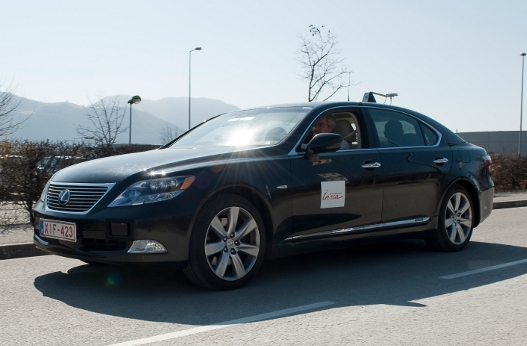
\includegraphics[width=0.55\columnwidth]{img/testbed:car}}\\
       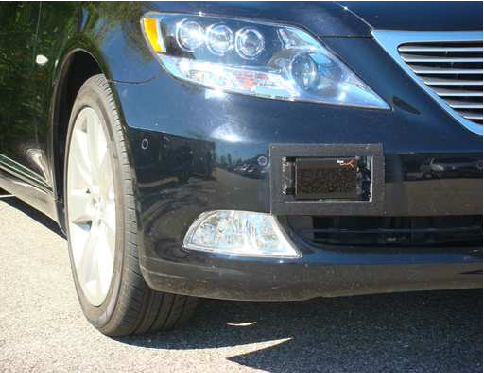
\includegraphics[width=0.40\columnwidth]{img/testbed:ibeo}
       &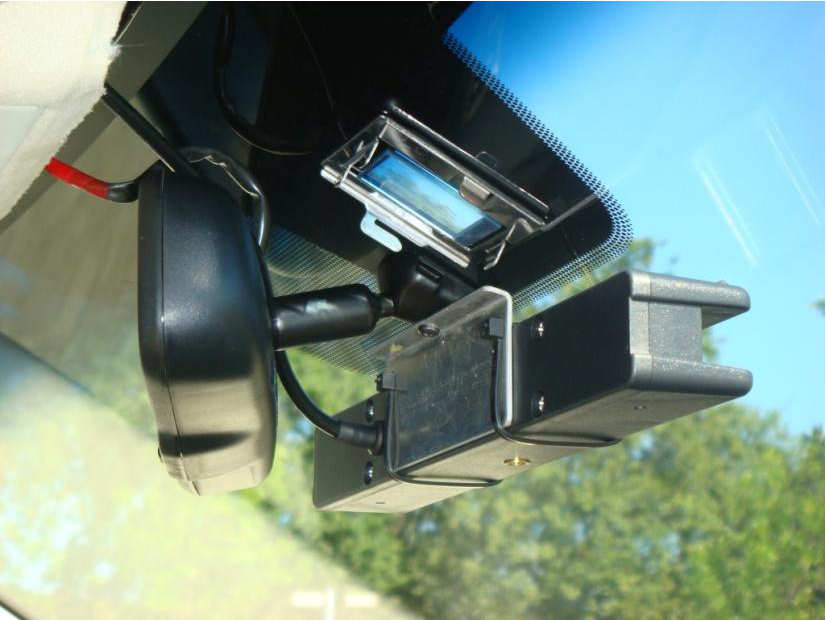
\includegraphics[width=0.40\columnwidth]{img/testbed:tyzx}
     \end{tabular}
   \caption{Lexus LS600h car equipped with two IBEO Lux lidars and a TYZX
     stereo camera}
   \label{fig:Lexus}
 \end{figure}

As the test platform requires a powerfull computer to process the stereo images in realtime, the car is equipped with a Dell workstation with an NVidia graphic card.

DeepSea TYZX stereo vision camera has a base line of 22 cm with 512x320 pixels of resolution and focal length of 410 pixels, this camera is provided with a library which can estimate the distance in cm of the objects captured by the camera, but in our tests we used the estimators developed at Inria\cite{PERROLLAZ-2010-493397}.
%better references
%http://ieeexplore.ieee.org/stamp/stamp.jsp?tp=&arnumber=6170895
%http://hal.inria.fr/index.php?halsid=fa9c2loot97ptftt2n38f6lvr5&view_this_doc=hal-00671208&version=1

\begin{figure}[h]
   \centering
     \begin{tabular}{lr}
       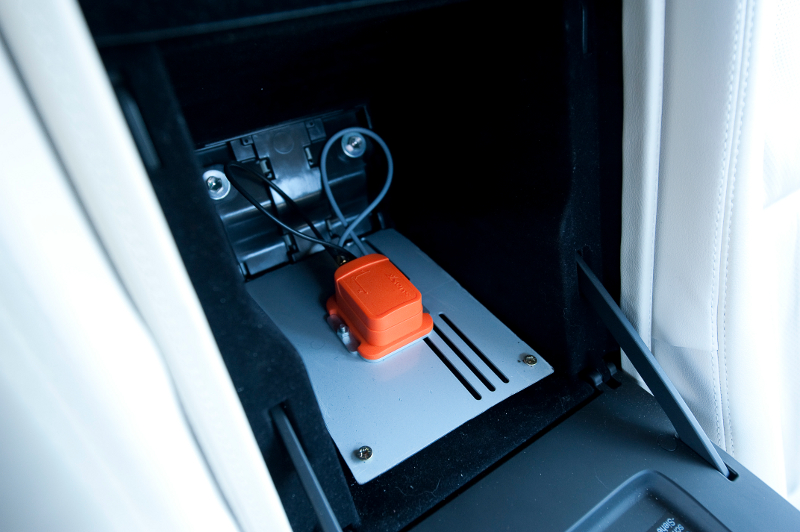
\includegraphics[width=0.45\columnwidth]{img/testbed:xsens}
       & 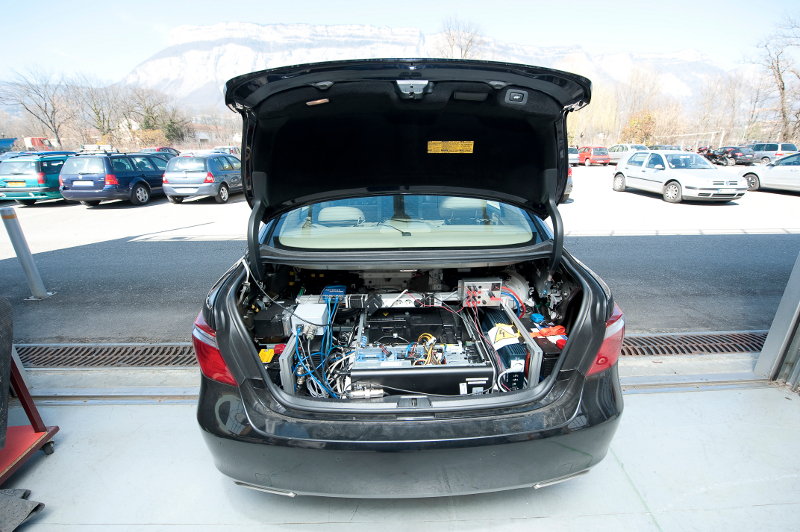
\includegraphics[width=0.45\columnwidth]{img/testbed:trunc}
     \end{tabular}
   \caption{MTi-G XSens IMU unit \& Intel Xeon 3.4GHz linux box}
   \label{fig:Lexus}
 \end{figure}

Each IBEO Lux Lidar is composed of four layers, each of them providing about 200 beams. The angular range of 100 degrees with angular resolution of 0.5 degrees. Each beam can reach until 200 m of distance measurement, with width of 40 m and maximum height of 2 m.

MTi-G XSens minimum of 120Hz and maximum of 512Hz for data logging and angular resolution of 0.05 degrees, all specifications are valid when considering an homogenous eletromagnetic environment. Maximum altitude operation is 18 Km and maximum speed is 515 m/s.



\subsubsection*{Software}

The high end cars are composed of several internal networks, each of them responsible to handle the transmission of the informations that are captured in that network to other one which need to process that information. This type of network is known as Controller Area Network (CAN) and provides a cheap and reliable way to communicate with devices, so CAN bus have been replacing the regular point-to-point wiring interconnection among the components\cite{bosch91can}.

Car manufacturers use platforms like YARP - Yet Another Robot Platform -, URBI or ROS to publish the information gathered by those networks, frameworks like ROS, allow the car to put the information into a shared memory array which can be access by other applications, the intent for most of those frameworks is to give longevity\cite{Fitzpatrick:2008:TLR:1327539.1327705} for the robot application that uses it by providing a platform that can evolve in cooperation manner with other projects.

For this project Robot Operating System(ROS) was adopted, ROS gives us the hability to save all information obtained during a run (driving the test platform) from all sensors, and replay it later in the laboratory, this by far allow to have a consistent test samples and a historical evolution of all scenarios gathered during the algorithm evolution, aloing the retro-performance benchmarking with other versions of the algorithm.

\subsubsection*{Assumptions}

\textit{Goal: What we assume to make our algorithm work}

\subsubsection*{Notation}

\paragraph{Occupancy Grid visual representation}

Representatiing the occupancy grid, implies in taking some precautions in the pattern used to represent each state, in this work the value $1$ represents occupied spaces and $0$ free spaces, although in the visual representation of the occupancy grid the $black$ dots represent occupied spaces and $white$ ones represent free spaces. In certain occasions, where the grid depicted is not binary, spaces where framework has absolutely no information about certain spaces (\textit{e.g.} due unreachability of the perception sensors in that sector), the color used is $gray$.

\subsection{Results}

\textit{Goal: What are our current results}

\subsection{Conclusion}

\textit{Goal: Express what we can conclude from this work, talk about future work, may be}